\section{Results}\label{sec:results}
Unless stated otherwise, the setting is $N=100$, observation level O3, $\tau=0$ and $\psi=1$ (B0 $=$ B1). Each IPPO run takes
about 10 minutes on 2 CPU threads ($2.4\times10^7$ household-steps). Numbers are mean $\pm$ s.d.\ across seeds, and every
entry is produced by \texttt{scripts/make\_report\_assets.py}.

\subsection{E1: Does decentralized learning recover the competitive equilibrium?}
\begin{table}[t]
\centering\small
\caption{E1 at $N=100$. B1-in-simulator executes the DP policy in the same finite-$N$ simulator with common random
numbers. W-loss: consumption-equivalent welfare loss relative to B1-in-simulator. DP-BR / PPO-BR: a single deviator's
consumption-equivalent gain (mean of the 10th, 50th and 90th wealth percentiles).}\label{tab:e1}
\resizebox{\linewidth}{!}{\begin{tabular}{lccccccccc}
\toprule
Policy & $\kappa$ & $K/N$ & hours & $a'/m$ & Gini & Top-10\% & W-loss (\%) & DP-BR (\%) & PPO-BR (\%)\\
\midrule
B1 (theory, $N{=}\infty$) & 8.713 & 2.953 & 0.333 & 0.840 & 0.549 & 0.342 & -- & -- & --\\
B1 in simulator & 8.745 & 2.955 & 0.333 & 0.840 & 0.545 & 0.337 & 0.00 & -0.01 & --\\
B2 (best constant) & 7.985 & 2.790 & 0.350 & 0.830 & 0.196 & 0.174 & 13.53 & 3.32 & --\\
Random & 0.889 & 0.442 & 0.500 & 0.495 & 0.513 & 0.352 & 3583.29 & -- & --\\
IPPO ($n{=}5$) & 7.532 $\pm$ 0.086 & 2.520 $\pm$ 0.032 & 0.334 $\pm$ 0.002 & 0.823 $\pm$ 0.001 & 0.464 $\pm$ 0.017 & 0.297 $\pm$ 0.007 & 1.36 $\pm$ 0.10 & 0.40 $\pm$ 0.07 & -0.00 $\pm$ 0.00\\
MAPPO ($n{=}5$) & 7.563 $\pm$ 0.122 & 2.530 $\pm$ 0.052 & 0.334 $\pm$ 0.002 & 0.824 $\pm$ 0.002 & 0.454 $\pm$ 0.010 & 0.291 $\pm$ 0.010 & 1.30 $\pm$ 0.19 & 0.42 $\pm$ 0.13 & 0.02 $\pm$ 0.05\\
\bottomrule
\end{tabular}
}
\end{table}
\begin{figure}[t]
\centering
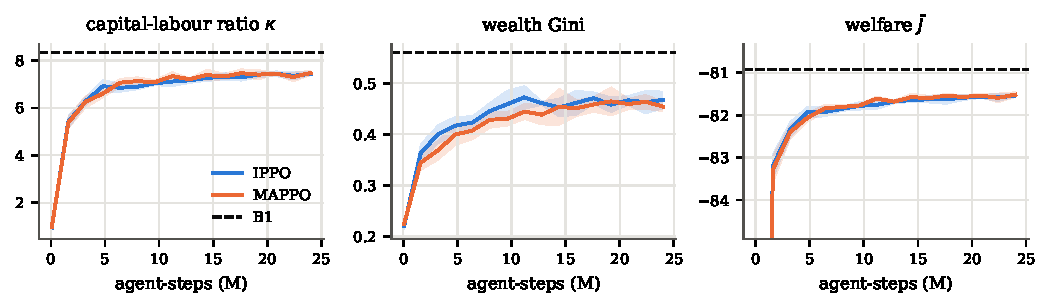
\includegraphics[width=\linewidth]{figures/fig_e1_learning.pdf}
\caption{E1 learning curves (5 seeds, mean $\pm$ s.d.), evaluated every 20 iterations with the deterministic
policy. Dashed: B1 executed under the same evaluation protocol.}\label{fig:e1learn}
\end{figure}
\begin{figure}[t]
\centering
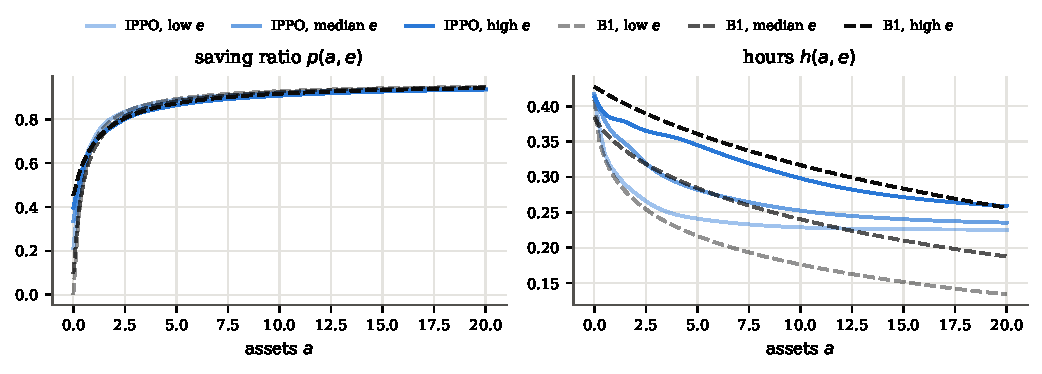
\includegraphics[width=\linewidth]{figures/fig_e1_policy.pdf}
\caption{Learned (IPPO seed 0) and B1 policy functions for low, median and high productivity, with the learner's
aggregate inputs fixed at their long-run means.}\label{fig:e1policy}
\end{figure}
\begin{figure}[t]
\centering
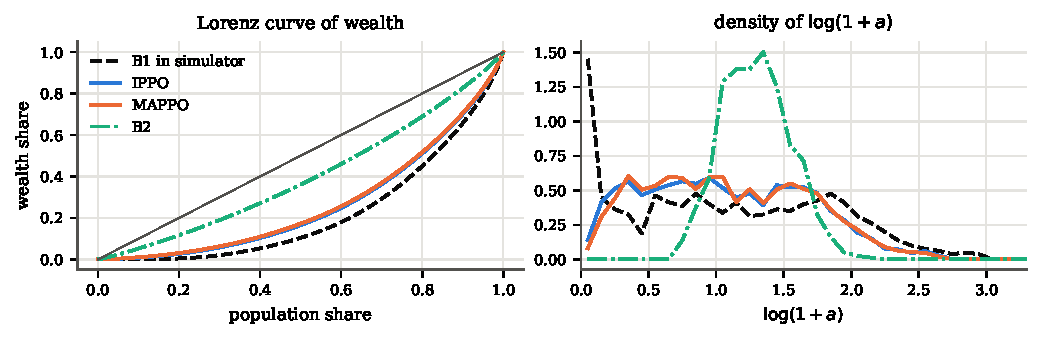
\includegraphics[width=\linewidth]{figures/fig_e1_wealth.pdf}
\caption{Stationary wealth distribution (pooled over seeds and 8 evaluation economies, $t=500$).}\label{fig:e1wealth}
\end{figure}

Table~\ref{tab:e1} and Figures~\ref{fig:e1learn}--\ref{fig:e1wealth} give the answer. \textbf{Aggregates.} Welfare
converges within 40 iterations ($3.2\times10^6$ household-steps) for both learners, while $\kappa$ keeps creeping up
slowly. The resulting stationary economy \emph{matches B1 in
labour supply exactly} (hours $0.334$ vs.\ $0.333$) but \emph{under-accumulates capital}: $\kappa=7.53\pm0.09$ (IPPO)
and $7.56\pm0.12$ (MAPPO) against $\kappa^\star=8.71$, a gap of $13.6\%$, which is about $35$ times the finite-$N$
gap of B1 itself ($0.4\%$). The interest rate is correspondingly higher ($3.9\%$ vs.\ $3.0\%$). \textbf{Policies.}
The saving-ratio function is learned closely (policy gap $0.047$; Figure~\ref{fig:e1policy}, left), and the remaining
error sits near the borrowing constraint, where poor households save too much and rich ones slightly too little. Hours
are learned less well: the learned wealth effect on labour is too weak, so wealthy low-productivity households
work $0.23$ instead of $0.14$. \textbf{Inequality.} The learned economy is markedly more equal (Gini $0.46$
vs.\ $0.55$, top-10\% share $0.30$ vs.\ $0.34$): it lacks both the mass of constrained households at $a=0$ and the
right tail (Figure~\ref{fig:e1wealth}). \textbf{Welfare.} The consumption-equivalent loss is only $1.36\pm0.10\%$
(IPPO) and $1.30\pm0.19\%$ (MAPPO). The best constant policy B2 loses $13.5\%$, so learning closes about $90\%$ of the
welfare gap between a naive rule and the equilibrium.

\textbf{Exploitability.} The learned profile is \emph{not} a Nash equilibrium. The exact DP best response to the
learned economy's prices gains $0.40\pm0.07\%$ consumption-equivalent (10th/50th/90th percentile: $0.42/0.26/0.53\%$).
As a sanity check, the same procedure gives $-0.01\%$ against B1 and $3.3\%$ against B2. By contrast, the PPO best
response (100 iterations, warm-started) finds essentially \emph{no} improvement ($0.00\%$ IPPO, $0.02\pm0.05\%$ MAPPO).
In 9 of 10 runs no checkpoint beats the warm-start policy on the validation snapshot. A model-free deviator thus misses
the gain that the model-based deviator finds, so learning-based exploitability estimates can badly understate the
distance to equilibrium.
\textbf{MAPPO vs.\ IPPO.} The centralized critic changes nothing measurable: every metric overlaps within one s.d.
This is consistent with the price-taking structure: with $N=100$ a household's value depends on the economy only
through two prices, which O3 already summarises.
\emph{Verdict on H1: supported.} MARL approaches B1 in labour supply and welfare, deviates by 14\% in capital,
and deviates most in the tails of the wealth distribution.

\subsection{E2: Does the gap shrink with population size?}
\begin{table}[t]
\centering\small
\caption{E2: population size (IPPO, O3). B1-sim gap: $|\kappa^{\rm B1\text{-}sim}-\kappa^\star|/\kappa^\star$, i.e.\ the
finite-$N$ error of the exact policy itself. Household-steps per run: $2.4\times10^7$ ($N\le100$), $1.8\times10^7$
($N=300$, one economy per iteration), $6\times10^7$ ($N=1000$).}\label{tab:e2}
\resizebox{\linewidth}{!}{\begin{tabular}{rcccccccc}
\toprule
$N$ & $n$ & $|\Delta\kappa|/\kappa^\star$ & B1-sim gap & $p$-gap & $h$-gap & W-loss (\%) & DP-BR (\%) & time (min)\\
\midrule
10 & 3 & 0.155 $\pm$ 0.008 & 0.023 & 0.065 $\pm$ 0.006 & 0.022 $\pm$ 0.003 & -1.54 $\pm$ 0.05 & -0.33 $\pm$ 0.04 & 7.6\\
30 & 3 & 0.154 $\pm$ 0.018 & 0.054 & 0.056 $\pm$ 0.005 & 0.016 $\pm$ 0.001 & 0.78 $\pm$ 0.13 & 0.86 $\pm$ 0.24 & 9.2\\
100 & 5 & 0.136 $\pm$ 0.010 & 0.004 & 0.047 $\pm$ 0.010 & 0.014 $\pm$ 0.001 & 1.36 $\pm$ 0.10 & 0.40 $\pm$ 0.07 & 9.8\\
300 & 3 & 0.156 $\pm$ 0.027 & 0.003 & 0.062 $\pm$ 0.011 & 0.019 $\pm$ 0.001 & 2.52 $\pm$ 0.29 & 1.08 $\pm$ 0.37 & 8.9\\
1000 & 3 & 0.088 $\pm$ 0.007 & 0.005 & 0.038 $\pm$ 0.008 & 0.012 $\pm$ 0.002 & 1.47 $\pm$ 0.03 & 0.18 $\pm$ 0.03 & 22.6\\
\bottomrule
\end{tabular}
}
\end{table}
\begin{figure}[t]
\centering
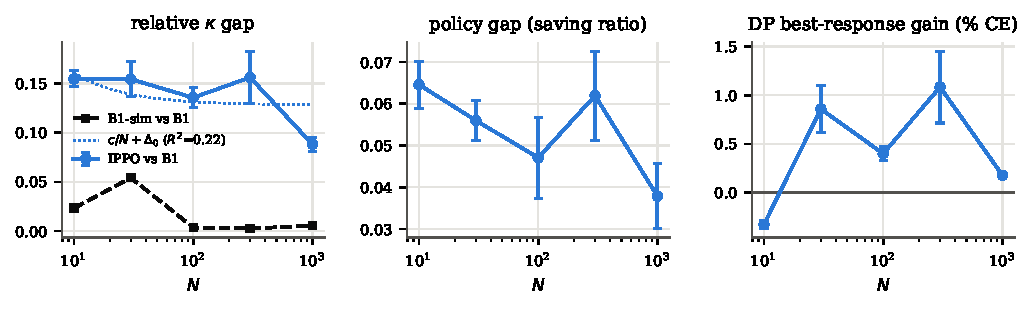
\includegraphics[width=\linewidth]{figures/fig_e2_population.pdf}
\caption{E2: capital gap with the fitted $c/N+\Delta_0$ curve, saving-policy gap and DP best-response gain versus $N$.}\label{fig:e2}
\end{figure}
H2 predicted $\Delta(N)\approx c/N+\Delta_0$. The data (Table~\ref{tab:e2}, Figure~\ref{fig:e2}) show that the
\emph{learning floor dominates}. The capital gap is $15.5\%$, $15.4\%$, $13.6\%$ and $15.6\%$ for
$N=10,30,100,300$, and $8.8\%$ for $N=1000$. The fit gives $\Delta_0=12.8\%$ with $R^2=0.22$ (a $c/\sqrt N$ fit does
no better, $R^2=0.33$). The gap is in fact ordered by the \emph{sample budget} rather than by $N$: the worst run
($N=300$) has the fewest household-steps and the best ($N=1000$) the most, so the $N=1000$ improvement cannot be
attributed to vanishing price impact. Price impact itself is visible only at the smallest $N$. At $N=10$, B1 executed
in the simulator \emph{loses} welfare relative to the learners (W-loss $-1.54\%$), and the DP best response computed at
mean prices is a \emph{worse} deviation ($-0.33\%$). With ten households prices fluctuate strongly (the s.d.\ of $\kappa$
across economies is $1.2$ under B1, against $0.16$ at $N=100$). A price-taking policy that ignores this volatility is
then no longer optimal, while learners adapt to the actual dynamics. For $N\ge30$ the known-model reference is the
better policy again. \emph{Verdict on H2: not supported at our training budget.} An $O(1/N)$ effect exists in the
benchmark itself (B1-sim gap) but is swamped by a ${\approx}13\%$ learning floor in MARL.


\subsection{E3: Does information help?}
\begin{table}[t]
\centering\small
\caption{E3: observation levels (IPPO, $N=100$). conv.\ iter: first evaluation reaching 95\% of the final welfare
improvement.}\label{tab:e3}
\begin{tabular}{lccccccc}
\toprule
Obs. & $n$ & $|\Delta\kappa|/\kappa^\star$ & $p$-gap & $h$-gap & W-loss (\%) & DP-BR (\%) & conv. iter\\
\midrule
O0 & 3 & 0.184 $\pm$ 0.002 & 0.044 $\pm$ 0.008 & 0.012 $\pm$ 0.001 & 1.21 $\pm$ 0.08 & 0.81 $\pm$ 0.05 & 33\\
O1 & 3 & 0.158 $\pm$ 0.016 & 0.036 $\pm$ 0.006 & 0.012 $\pm$ 0.002 & 1.27 $\pm$ 0.27 & 0.49 $\pm$ 0.17 & 27\\
O2 & 3 & 0.157 $\pm$ 0.003 & 0.037 $\pm$ 0.006 & 0.012 $\pm$ 0.000 & 1.19 $\pm$ 0.06 & 0.48 $\pm$ 0.05 & 33\\
O3 & 5 & 0.136 $\pm$ 0.010 & 0.047 $\pm$ 0.010 & 0.014 $\pm$ 0.001 & 1.36 $\pm$ 0.10 & 0.40 $\pm$ 0.07 & 40\\
\bottomrule
\end{tabular}

\end{table}
Table~\ref{tab:e3} shows that information matters for \emph{aggregates and exploitability} but
not for welfare. Adding lagged prices (O0$\to$O1) cuts the capital gap from $18.4\%$ to $15.8\%$ and the DP best-response
gain from $0.81\%$ to $0.49\%$. Without prices a household cannot condition on the return to saving, so it
under-reacts to it. Aggregate capital and labour (O2) add nothing beyond prices, which is expected because in a
competitive economy prices are sufficient statistics for aggregates. The TaxAI group statistics (O3) reduce the gap
further to $13.6\%$ and the exploitability to $0.40\%$. The welfare loss is flat at $1.2$--$1.4\%$ across all levels,
so most of the welfare comes from the individual state $(a,e)$, which every level observes. All levels converge within
about 40 iterations. \emph{Verdict on H3: partially supported.} Prices (O1) help as predicted, but O2 adds nothing
while O3 still helps, the opposite of the predicted ordering.

\subsection{E4: Do learners respond to taxes like the equilibrium?}
\begin{table}[t]
\centering\small
\caption{E4: proportional income tax $\tau$ with revenue wasted ($\psi=0$) or rebated lump-sum ($\psi=1$). IPPO, O3,
3 seeds. B1 columns are the exact stationary equilibrium.}\label{tab:e4}
\resizebox{\linewidth}{!}{\begin{tabular}{ccccccccc}
\toprule
$\tau$ & $\psi$ & $K/N$ MARL & $K/N$ B1 & hours MARL & hours B1 & Gini MARL & Gini B1 & $\bar J$ MARL / B1\\
\midrule
0.1 & 0 & 2.327 $\pm$ 0.012 & 2.798 & 0.336 $\pm$ 0.002 & 0.338 & 0.454 & 0.538 & -85.8 / -85.3\\
0.2 & 0 & 2.193 $\pm$ 0.048 & 2.620 & 0.342 $\pm$ 0.001 & 0.342 & 0.468 & 0.531 & -90.6 / -89.9\\
0.3 & 0 & 1.985 $\pm$ 0.034 & 2.417 & 0.351 $\pm$ 0.001 & 0.348 & 0.477 & 0.523 & -96.3 / -95.5\\
0.0 & 1 & 2.520 $\pm$ 0.032 & 2.953 & 0.334 $\pm$ 0.002 & 0.333 & 0.464 & 0.545 & -81.8 / -81.3\\
0.1 & 1 & 2.218 $\pm$ 0.048 & 2.632 & 0.320 $\pm$ 0.002 & 0.321 & 0.460 & 0.551 & -81.2 / -80.6\\
0.2 & 1 & 1.943 $\pm$ 0.015 & 2.306 & 0.307 $\pm$ 0.001 & 0.307 & 0.481 & 0.556 & -80.8 / -80.1\\
0.3 & 1 & 1.650 $\pm$ 0.029 & 1.976 & 0.291 $\pm$ 0.000 & 0.294 & 0.473 & 0.563 & -80.9 / -80.0\\
\bottomrule
\end{tabular}
}
\end{table}
\begin{figure}[t]
\centering
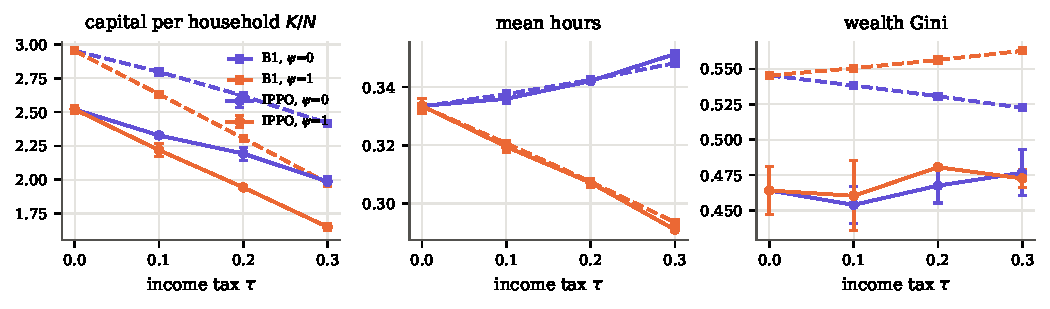
\includegraphics[width=\linewidth]{figures/fig_e4_tax.pdf}
\caption{E4: capital, hours and wealth Gini versus $\tau$. Solid: IPPO (mean $\pm$ s.d.); dashed: B1 equilibrium.}\label{fig:e4}
\end{figure}
The tax experiment is the strongest result (Table~\ref{tab:e4}, Figure~\ref{fig:e4}). \textbf{Signs.} MARL reproduces
every qualitative prediction of the equilibrium. Capital falls with $\tau$ in both regimes. Hours \emph{rise} with
$\tau$ when revenue is wasted, because the income effect dominates when households are poorer. Hours \emph{fall} when
revenue is rebated, because the substitution effect dominates once the rebate removes the income effect. The rebate
regime cuts capital more. \textbf{Magnitudes.} The elasticities with respect to the net-of-tax rate are close to B1's:
$\varepsilon_K=0.65$ vs.\ $0.56$ and $\varepsilon_h=-0.15$ vs.\ $-0.12$ ($\psi=0$); $\varepsilon_K=1.18$ vs.\ $1.13$
and $\varepsilon_h=0.38$ vs.\ $0.36$ ($\psi=1$). Hours match B1 to within $0.003$ in every regime. The capital shortfall is
a nearly constant \emph{level} effect: learned $\kappa$ is $83$--$86\%$ of $\kappa^\star$ in all seven regimes, so it
largely cancels in comparative statics. \textbf{Where MARL fails.} Inequality responds to taxes with the wrong
sensitivity. In B1, the rebate raises the Gini (from $0.545$ to $0.563$) because the lump sum makes low-wealth
households less willing to save, and wasted revenue lowers it. MARL's Gini stays at $0.45$--$0.48$ with no clear trend
in either regime. In $13$ of the $49$ runs (mostly $\tau\ge0.2$ and O0), under-saving pushes the after-tax return
above $1/\beta$, which is impossible in a stationary equilibrium; there we use the 200-period finite-horizon DP best
response. \emph{Verdict on H4: supported} for signs and, unexpectedly, for magnitudes of aggregate responses; not
supported for distributional responses.

